%
%
%

\chapter{Feedback}\label{FeedbackChapter}

\section{Problem Statement and Learning Objectives}
Be able to

\begin{itemize}
    \item Explain the difference between signal and energy flows in dynamical systems.
    \item Explain the precise meaning of a block in a signal flow block diagram and
    perform basic block diagram transformations.
    \item  Derive the end-to-end closed-loop gain of a system with negative feedback.
    \item Explain the ``loop gain" of a system with negative or positive feedback.
    \item Define Sensitivity Analysis and be able to numerical compute sensitivity of
    a defined performance parameter to a system parameter.
    \item Define Disturbance Rejection and explain how Disturbance Rejection depends on
    loop gain.
    \item Compute and Bode Plot  Disturbance Rejection for disturbances at various locations in the system.
    \item Numerically compute poles and zeros (with software) of the open and closed loop gains and determine whether or not the system is stable.
    \item Evaluate gain and phase in the frequency domain to determine system stability.
    \item Compute (graphically from hand drawn Bode plots) and explain significance of Gain and Phase Margin.
\end{itemize}

\section{Block Diagram Transformations}

\subsection{Signals vs. Energy Flows}

A key distinction in understanding systems is that between {\it signals} and {\it energy flows}.


\begin{itemize}
  \item  A {\it signal} is a variable which carries information but does not directly regulate the exchange of energy.

For example,  a voltage, $V(t)$ which varies with time, carries some information.   This voltage may be applied to a system component as an input but we will only call this a {\it signal} if the corresponding input current is zero (or negligible).  In this case the input power is always zero.

  \item  An {\it energy flow} is the case where a non-zero power flows into or out of the connection.
\end{itemize}

\begin{ExampleSmall}
Classify the following situations into signals vs. energy flows:

\begin{enumerate}
  \item  A voltage $V_1(t)$ is connected to a resistor of 50 $\Omega$.

  $V_1(t)$  is part of an energy flow since the current in general is non zero.

  \item A voltage $V_2(t)$ is connected to an amplifier with a high impedance input ($i_{in} \approx 0$).

  $V_2(t)$ can be considered a signal since there is no power flow ($P=V_2(t)\times i_2(t) = 0$).


  \item A force, $f_3(t)$ is applied to a translational dynamical system consisting of intertia, damping, and spring, and the system responds.

  $f_3(t)$ is part of an energy flow since the velocity, $\dot{x}(t)$ is non zero, and therefore the mechanical power,
  $P = f(t)\times \dot{x}(t) \neq 0$.

\end{enumerate}

\end{ExampleSmall}


While it is possible to simulate energy flows using signals and block diagrams, this case will not be considered further.



\subsection{Block Diagrams}
The basic idea of a block diagram is familiar to most people but there are a few subtleties.  A block maps one signal to another.  A single block (Figure \ref{singleblock}), has an equivalent equation

\bq\label{blockequation}
Y(s) = G(s)X(s) \qquad \mathrm{or} \qquad G(s) = \frac{Y(s)}{X(s)}
\eq
In other words, the block is a graphical representation of multiplication of a Laplace Transform of a signal by the Laplace Transform of a transfer function.


\begin{figure}\centering
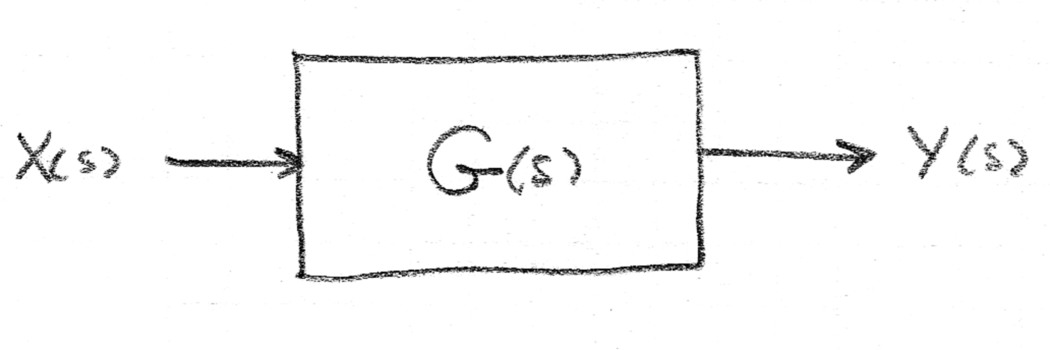
\includegraphics[width=3.5in]{figs06/00764a.png}
\caption{A single block,}\label{singleblock}
\end{figure}


\begin{ExampleSmall}
Find the expression for $Y(s)$

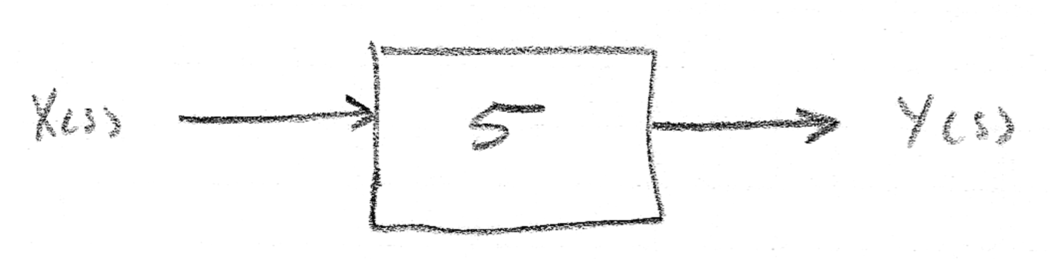
\includegraphics[width=3.5in]{figs06/00765a.png}

\[
Y(s) = 5 X(s)
\]

\end{ExampleSmall}


\begin{ExampleSmall}
Find the expression for $B(s)$ and $b(t)$

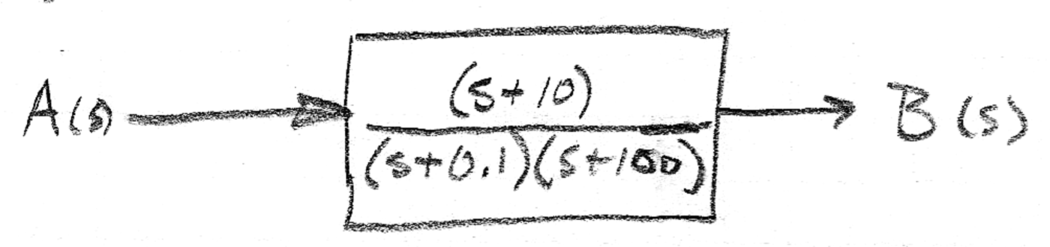
\includegraphics[width=3.5in]{figs06/00766a.png}

\[
B(s) = \frac{A(s)(s+10)}{(s+0.1)(s+100)}
\]

\[
b(t) = \mathcal L^{-1} \left \{ \frac{A(s)(s+10)}{(s+0.1)(s+100)}  \right \}
\]
\end{ExampleSmall}

One consequence of these definitions, is that there is no influence of the output of a block on its input.
Put another way, there is no ``loading" of an output by any number of subsequent inputs.


\subsection{Transformations}

When blocks are combined into block diagrams, the definitions above can easily be applied to figure out the meaning of the particular combination.  Connections include (Figure \ref{serialparallelblocks}):

Series: the output of the first block is connected to the input of a second block.

Parallel:  The output is the sum of the outputs of two blocks with the same input.

\begin{figure}\centering
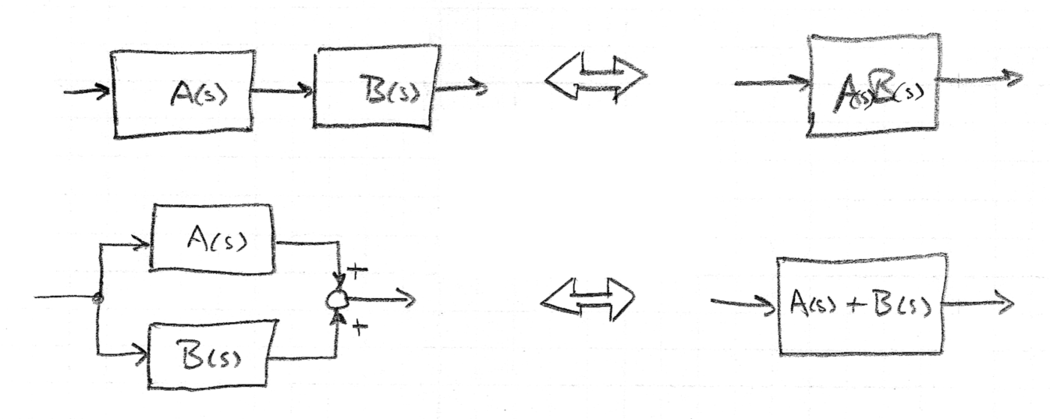
\includegraphics[width=3.5in]{figs06/00767a.png}
\caption{Series and parallel connections of blocks.}\label{serialparallelblocks}
\end{figure}

Some tranformations are slightly less obvious, but arise easily from Equation \ref{blockequation} as well as the properties of linearity.

The simple relationships
\[
A(s) \left ( x(s)+ y(s) \right) \Leftrightarrow A(s)x(s) + A(s) y(s)
\]

and
\[
y_1(s) = A(s) x(s), \quad y_2(s) = y_1(s)  \Leftrightarrow  y_1(s) = A(s)x(s), \quad y_2(s) = A(s)x(s)
\]

Can be used to manipulate block diagrams as shown in Figure \ref{blocktransforms}

\begin{figure}\centering
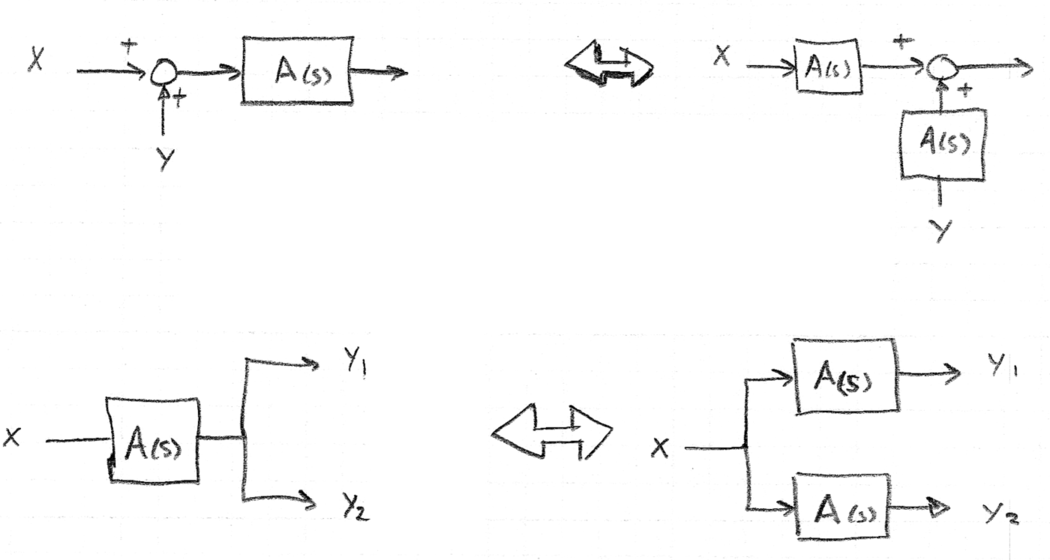
\includegraphics[width=3.5in]{figs06/00768a.png}
\caption{Block diagram transformations.}\label{blocktransforms}
\end{figure}

\section{Closed Loop Negative Feedback Gain}

\begin{figure}\centering
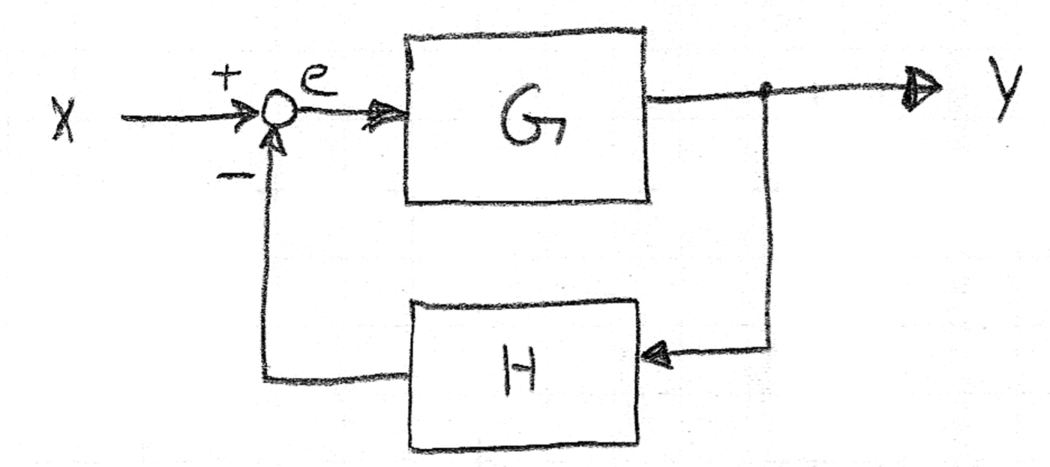
\includegraphics[width=3.5in]{figs06/00769a.png}
\caption{The closed loop negative feedback system.}\label{closedloopnegfeedbackblockdiag}
\end{figure}

One block diagram has supreme importance in control systems design (Figure \ref{closedloopnegfeedbackblockdiag}).  This is called the ``closed loop negative feedback system."   As implied by its name, the connections of the diagram form a loop, the loop contains a minus sign, and the output is ``fed back" to be subtracted from the input.

Even though this diagram is fairly simple, it is slightly more subtle to figure out an equivalent single block.  In other words, can we figure out an expression for $Y(s)/X(s)$ from the block diagram of Figure \ref{closedloopnegfeedbackblockdiag}?
The key is identifying the output of the summation and giving it the name, $E(s)$, which stand for error.  This term is called ``error" because it is the difference between input and output.  For example, if the closed loop negative feedback system were used to model a temperature control system, and the input was 68 degrees but the output (room temperature) was 72 degrees, then (with the frequently used assumption that $H=1$) the error would be -4 degrees.  Thus
\[
E(s) = X(s)-Y(s)H(s)
\]
Using block diagram relationships and dropping the $(s)$ for convenience
\[
Y = GE = G(X-YH)
\]
\[
Y = GX-GHY
\]
\[
Y(1+GH) = GX
\]
\bq\label{hsblackeqn}
\frac{Y}{X} = \frac {G} {(1+GH)}
\eq
This expression is called the closed loop transfer function.  It was discovered by H.S. Black of Bell Labs in 1927.

A common application of Figure \ref{closedloopnegfeedbackblockdiag} is a feedback control system in which $G(s)$ represents a combination of a controller and a plant.  The controller (typically implemented today with a microcontroller and associated I/O devices) generates a command signal to the plant which is the system to be controlled.  The feedback element $H$ is usually some kind of sensor which measures the output such as a temperature sensor or tachometer.  In many control systems $H=1$ since the objective is eliminating error betweeen the desired output ($X$) and the actual output ($Y$).


An important case is when $|GH| >> 1$.   Applying this to Equation \ref{hsblackeqn},
\[
\frac{Y}{X} \approx 1/H
\]
The quantity $GH(s)$ is called the {\it loop gain}.   In more complex block diagrams, the loop gain is the product of all blocks around the loop.
Expressed as a block diagram transformation, HS Black's equation (Eqn \ref{hsblackeqn}) is shown in Figure \ref{hsblacktransforms}.


\begin{figure}\centering
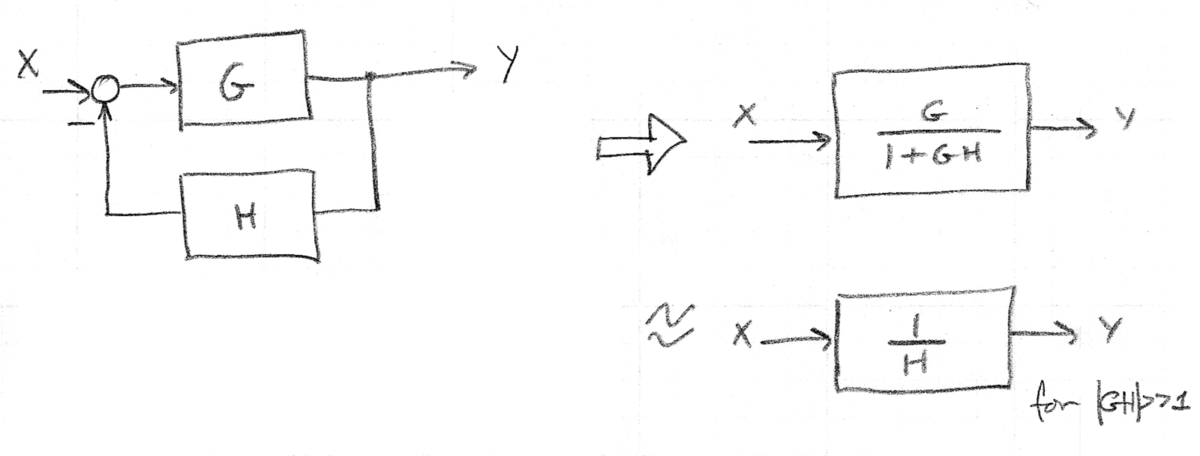
\includegraphics[width=4.0in]{figs06/00770a.png}
\caption{Equation \ref{hsblackeqn} expressed as a block diagram transformation.}\label{hsblacktransforms}
\end{figure}




\begin{ExampleSmall}
For the following system,

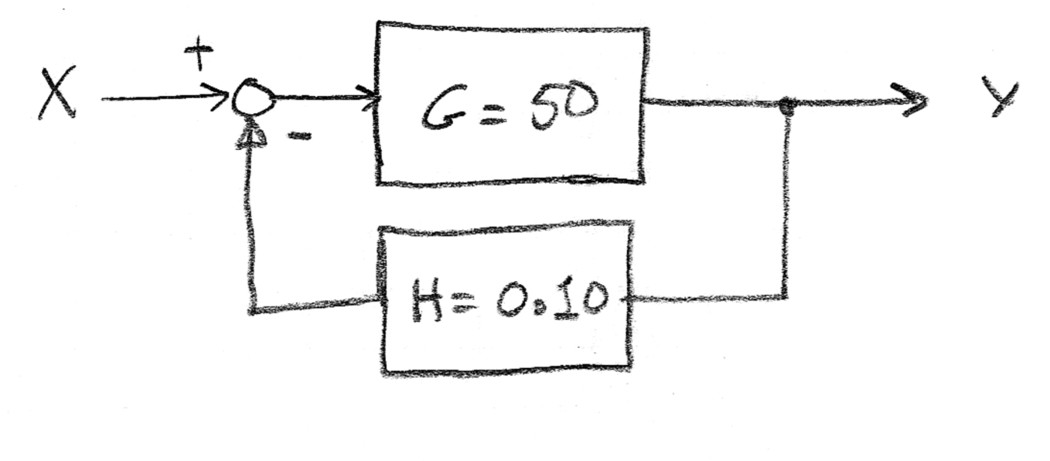
\includegraphics[width=3.5in]{figs06/00771a.png}

Find $\frac {Y}{X}$

\[
\frac{Y}{X} = \frac {G} {1+GH} =  \frac {50 }   {1+0.1\times 50} = 8.33
\]


\vspace{0.2in}
What if $G = \{100, 500, 10^5\}$ ?

\vspace{0.1in}
\begin{tabular}{|c|c|c|} \hline
$G$         & $Y/X$      &  $GH$   \\ \hline
 100        & $\frac{100}{1+0.1\times100 } = 9.09$      &  $10>1$        \\ \hline
 500        & $\frac{50}{51} = 9.80$                    &  $50 > 1$      \\ \hline
 $10^5$     & $\frac{10^5}{1+10^4} = 9.9999$            &  $10^4 >> 1$   \\ \hline
\end{tabular}

\vspace{0.05in}
As $GH$ gets larger in magnitude, $Y/X$ gets closer and closer to $1/H$.

In this example, $H<1$.  While $H=1$ is more typical for control systems, the situation
where $H<1.0$ is very often used in amplifiers such as audio amplifiers (HS Black's application).

\end{ExampleSmall}


As we will see in detail in the next sections, the behavior of closed loop negative feedback systems when $GH>>1$ has major engineering advantages including:


\begin{itemize}
  \item Reduced sensitivity to parameter variations.
  \item Ability to reject external disturbances.
\end{itemize}




\section{Sensitivity Analysis} The performance of a system depends on all of its
parts, but which parameters are most important in determining performance?
Sensitivity analysis is a way to answer that question.  Often a low precision
component costs much less than a high precision version of the same component.
If the sensitivity of performance to a parameter is low, then use of a low
precision component should have a small  effect on performance and cost can be
saved.  Conversely, if sensitivity of performance to a different parameter is
high, then a variation of its parameter value will make a big impact on
performance which might justify the additional cost of a precision component.

We will call some measure of system performance, $P$.   If a system has multiple
performance measures, we use $P_i$ to designate one of them.  The parameters of
a model of the system will be $p_i$.   With these definitions, we define
Sensitivity of performance measure $i$ to parameter $j$, about the current
values, ${p_{j0}},{P_{i0}}$, as

\begin{equation}
S_{ij} = \frac {\Delta P_i}{\Delta p_j } \frac{p_{j0}}{P_{i0}}
\end{equation}
This is like a derivative, but it is normalized by the values of the parameter and performance measure.
Qualitatively, sensitivity can be thought of as
\[
S_{ij} = \frac {\mathrm{\%\quad change\quad in\quad performance}_i}  {\mathrm {\%\quad change\quad in\quad parameter}_j}
\]

Although sensitivity can be derived analytically, we will concentrate here on using a numerical method.

\begin{ExampleSmall}\label{sensexample}
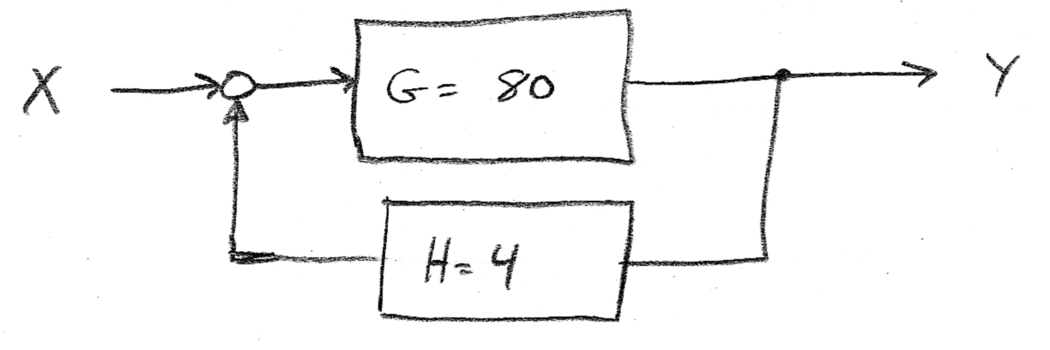
\includegraphics[width=3.5in]{figs06/00772a.png}

One aspect of performance is the gain or magnitude ratio, $\left |\frac{Y}{X} \right|$.  Find the sensitivity of $P_i = \left |\frac{Y}{X} \right|$ to the parameter $G$.   In other words, compute sensitivity for
\[
P_i = \left |\frac{Y}{X} \right| \qquad p_j = G
\]
Choose $\Delta = 10\%$.  We'll tabulate values of $G$, $H$, and $P_i$ in order to compute $S_{ij}$.

\vspace{0.2in}
\begin{tabular}{ccr} \hline
 $G$   &  $H$   &  $P_i$       \\ \hline
  80   &   4    & $\frac{80}{1+4\times80} = \frac{80}{321} = 0.24922$     \\ \hline
  88   &   4    & $\frac{88}{1+4\times88} = 0.24929$                      \\ \hline
\end{tabular}

\vspace{0.2in}
Now we compute $\Delta P_i$ by subtracting the numerical results (note that we need to use 6 significant figures to get a non-zero result).
\[
\Delta P_i = 0.24929 - 0.24922 = 0.00007 = 7.0\times10^{-5}
\]
Therefore,
\[
S_{ij} = \frac{7\times10^{-5}/0.24922}{8/80} = 2.81\times10^{-3} = 0.3\%
\]
Since sensitivity values are normalized by the nominal values of parameter and performance, we can judge them on an absolute scale where $S_{ij} =100\%$ indicates strong sensitivity.   In this case we can see that sensitivity of closed loop gain to $G$ is small.

\end{ExampleSmall}


\begin{ExampleSmall}
Find the sensitivity of the system of Example \thechapter.\ref{sensexample} to $H$


\vspace{0.2in}
\begin{tabular}{ccr} \hline
 $G$   & $H$  &  $P_i$       \\ \hline
  80   & 4    &  $\frac{80}{1+4\times80} =   0.24922$     \\ \hline
  80   & 4.4  &  $\frac{80}{1+4.4\times80} = 0.22662$                      \\ \hline
\end{tabular}
\vspace{0.2in}

\[
\Delta P_i = 0.22662 - 0.24922 =  -0.02259
\]
Therefore,
\[
S_{ij} = \frac{\frac{-0.02259}{0.24922}}{0.4/4} = -0.906 = -91\%
\]

This is a high degree of sensitivity.  A negative value for $S_{ij}$ means that the performance goes down when the parameter goes up.
\end{ExampleSmall}

 The important point of the previous two examples is that performance of the closed loop negative feedback system depends strongly on $H$ but weakly on $G$ (especially as $|GH| >>1$).


\section{Disturbance Rejection}

Another important aspect of control system performance is rejection of external disturbances.  External disturbances are unwanted inputs injected from the environment into a system.   {\it Disturbance rejection} is the amount by which a disturbance input to the system is reduced at the system output.

\begin{ExampleSmall}
Give two examples of disturbances in control systems.  Identify the inputs and outputs and explain what is the disturbance signal.

1) Consider an automatic pilot on a commercial aircraft.  The input to the automatic pilot is the desired heading in degrees relative to North. The output of the system is the plane's actual heading, for example as sensed by a compass.   Gusts of wind which blow the plane off its heading constitute an external disturbance.

2) Consider the temperature control system for a refrigerator.  The input is the desired temperature (such as a constant value of 38 deg F.). The system output is the actual temperature inside the refrigerator.   When the door is opened there is an input of warm air which increases the air temperature.  This increase in temperature is   a disturbance.
\end{ExampleSmall}


\begin{figure}\centering
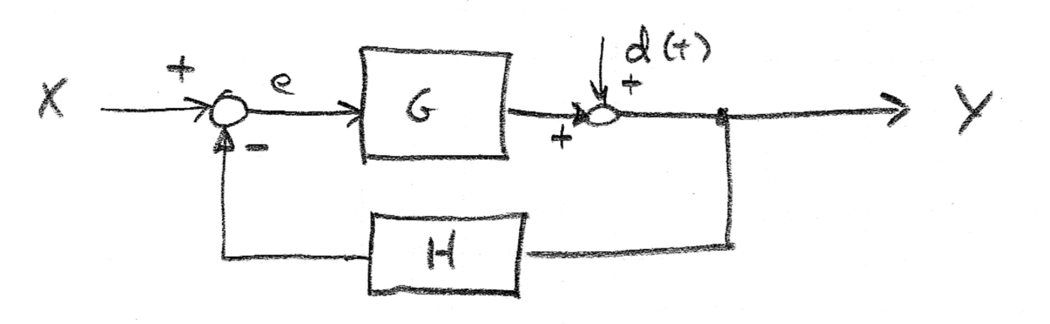
\includegraphics[width=3.5in]{figs06/00773a.png}
\caption{A closed loop system with a disturbance.}\label{DisturbanceLoop}
\end{figure}


The block diagram of Figure \ref{DisturbanceLoop} is a representation of a closed loop negative feedback system with a disturbance, $d(t)$.
Let's calculate the output, $Y$.

\[
Y = D + EG
\]
\[
Y = D+ G(X-YH)
\]
\[
Y(1+GH) = D+GX
\]
\bq\label{disturbanceoutput}
Y = \frac{D}{(1+GH)} + \frac{G }{(1+GH)} X
\eq

 The output thus consists of two components, one due to the disturbance, $D$, and one due to the input, $X$.   Note what happens however when $GH>>1$. In that case
 \[
 Y \approx D/GH + X \frac{1}{H}
 \]

 The disturbance input is {\bf reduced by the loop gain, $GH$}.

\paragraph{Disturbance Examples}

There are many phenomena which can be treated as disturbances in analysis of a control system and thus reduced by Equation \ref{disturbanceoutput}.
Some frequently encountered disturbances include:


\begin{itemize}
  \item Electrical Noise (additive)
  \item Unmodeled mechanical effects such as non-linear friction, or effects of temperature on mechanical parameters.
  \item Parameter value changes
  \item Vibrations
  \item Unmodeled flexibility or mechanical resonance.
\end{itemize}



\begin{Example}
Illustrate  how a non-linear spring could be broken down into a linear spring plus a disturbance.

Suppose our spring obeys
\[
f(x) = Kx + 0.1Kx^2
\]

Notice that this can be broken down into a linear part ($Kx$) and nonlinear part ($0.1Kx^2$).  One approach might be simply to separate the linear from the non linear terms above.  As shown in the plot below, a different split gives a higher stiffness to the linear term in such a way as to make a smaller non-linear term.

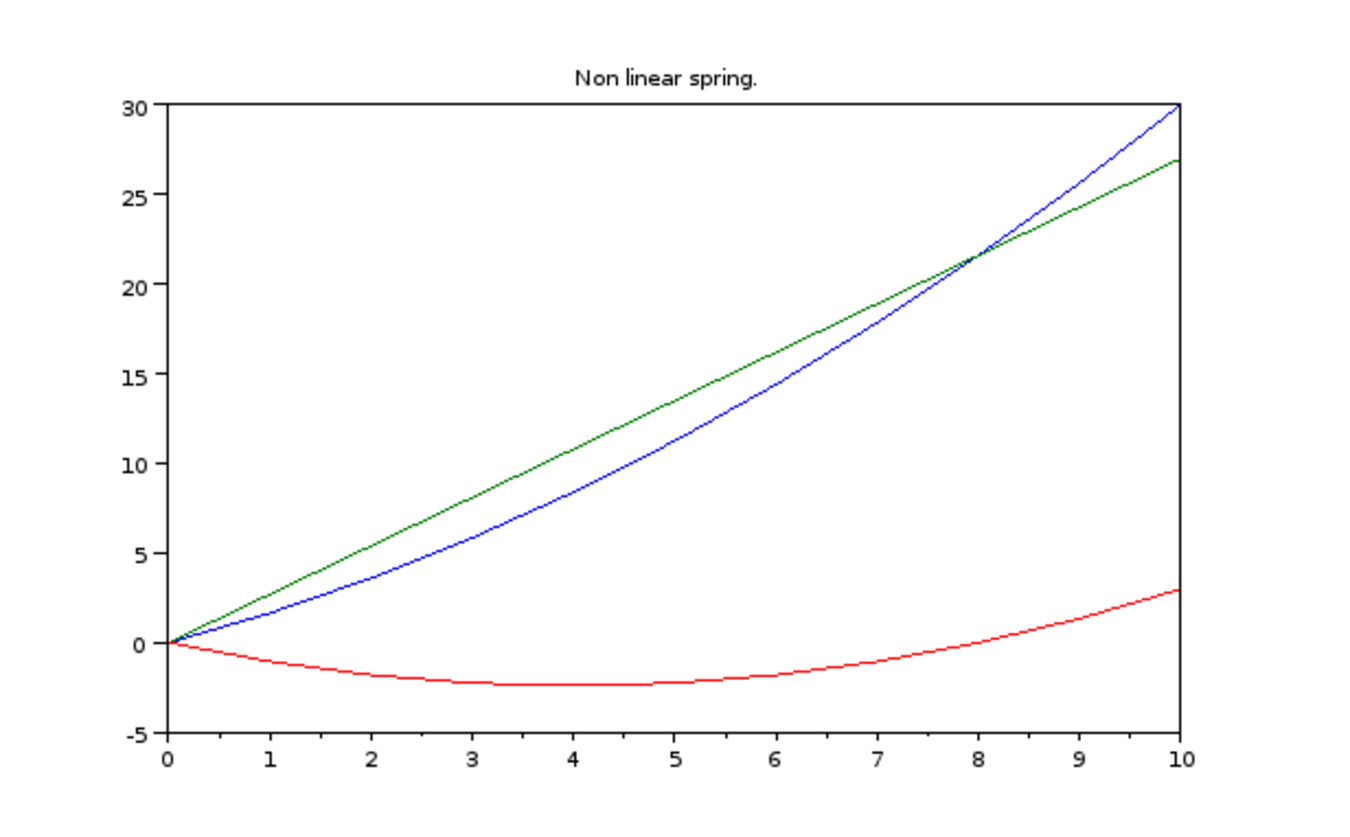
\includegraphics[width=4.5in]{figs06/nlspringa.png}



This computer plot shows the nonlinear spring given by the equation above and $K=1.5$ and also (in green) a linear fit:
\[
f(x) = 2.7x
\]

The difference
\[
f_{NL} = Kx + 0.1Kx^2 - 2.7x
\]
is shown in red. Note that we have ``linearized'' the spring function with a different approach to that of Chapter 1.   Using Chapter 1's method, we will get a better fit to one {\it specific point} on the curve (the point at which we compute linearization), but the green line above gives us a different kind of linearization which works over a broad range of $x$ values (and itersects at $two$ points).  Such a line could be computed, for example, by linear regression.



Suppose the system goes through a trajectory,
\[
x(t) = 5+5\sin(5t)
\]

Then this nonlinear spring would generate the following forces:

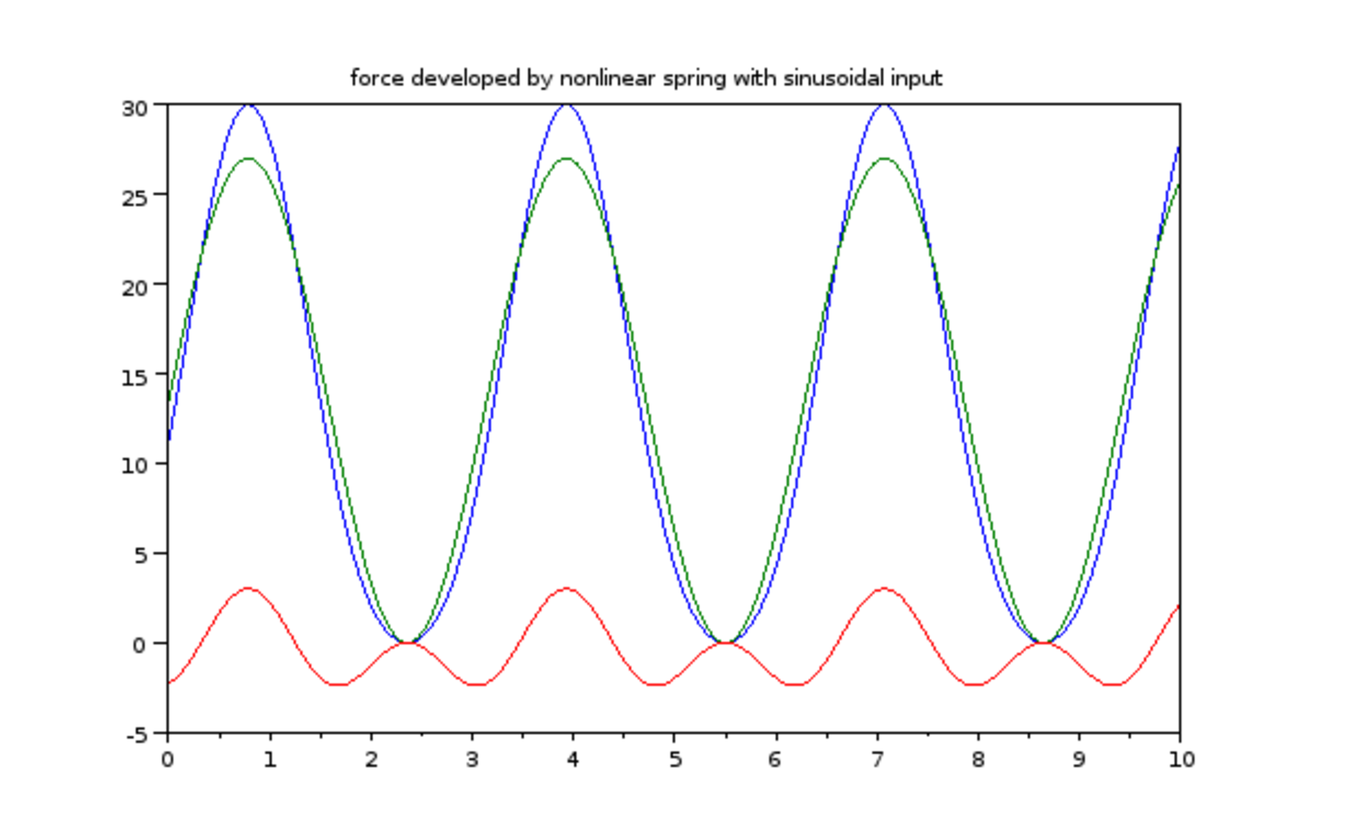
\includegraphics[width=4.5in]{figs06/fsinnlspringa.png}

Here the sinusoidal force output is nonlinear (blue) but can be broken down into a linear part (green) and a non-linear part (red). The linear approximation is pretty good (for this system at least) and the non-linear forces (red) can be treated as a disturbance (which is then attenuated by Equation \ref{disturbanceoutput}).

\end{Example}


\subsection{Disturbance Rejection in the Frequency Domain}


\begin{ExampleSmall}

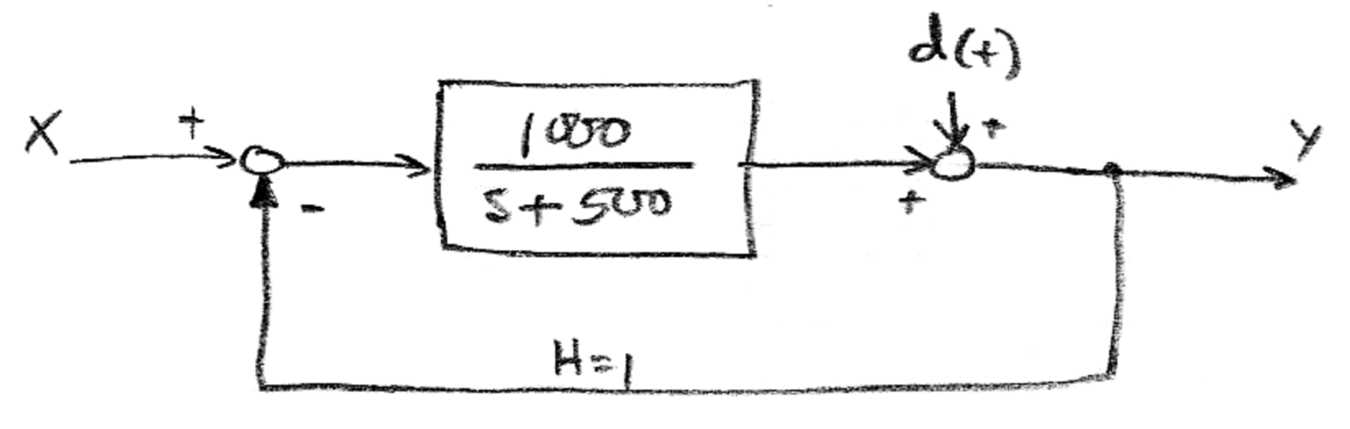
\includegraphics[width=4.5in]{figs06/00774a.png}

Find
\[
\frac{Y(s)}{D(s)} \quad \mathrm{for} \quad  X(s) = 0
\]
and sketch the BAMP of $GH(j\omega)$ and $\frac{Y(j\omega)}{D(j\omega)}$.

\vspace{0.25in}

\[
\frac{Y(s)}{D(s)} = \frac{1}{1+GH} =  \frac  {s+500}  {s+500 + 1000} = \frac{(s+500)}{(s+1500)}
\]
and
\[
GH(s) = \frac{1000}{(s+1500)}
\]


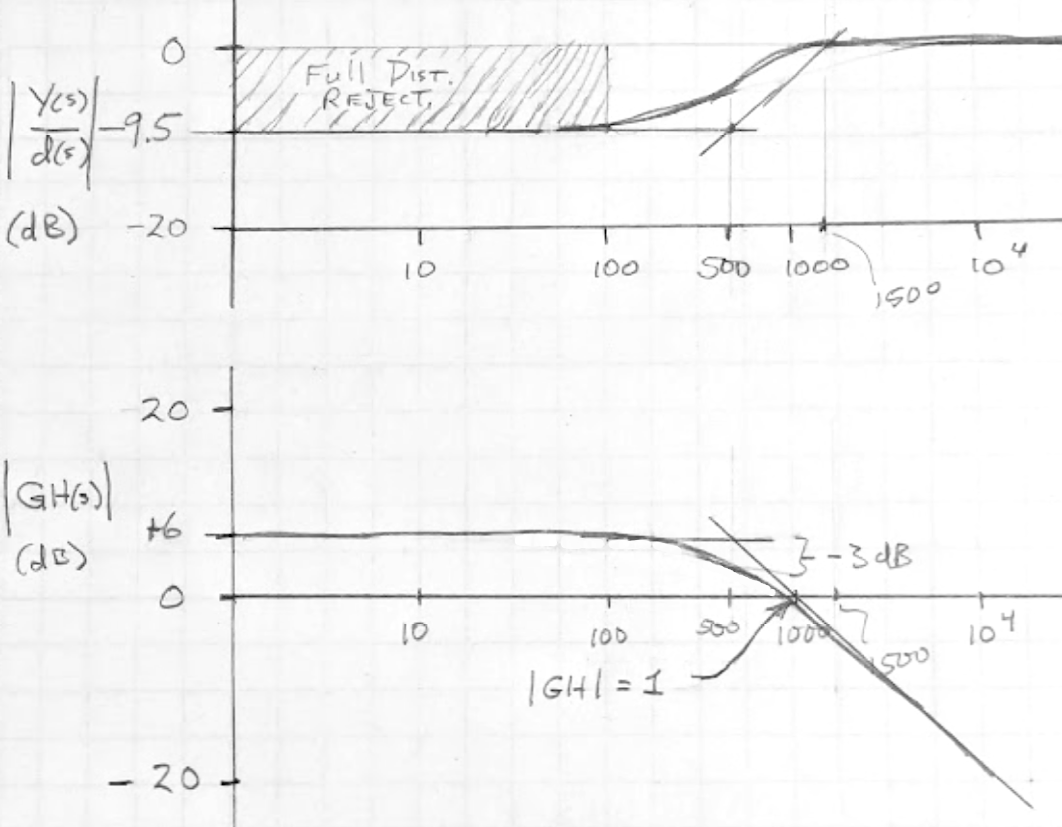
\includegraphics[width=4.5in]{figs06/G64M22.png}


The disturbance rejection is -9.5$dB$ for frequencies below about 100 rad/sec.   There is
little or no disturbance rejection above about 1000 (which is the point where loop gain
magnitude is 1.0). (margin values in paren represent computer results for $GH(s)$.)

\end{ExampleSmall}

\subsection{Location of Disturbance}

Disturbances can enter the control loop at different locations besides summing with the output.  First consider the disturbance injected into the error computation (e.g, a noisy sensor, Figure \ref{disturbanceaterror}).


\begin{figure}\centering
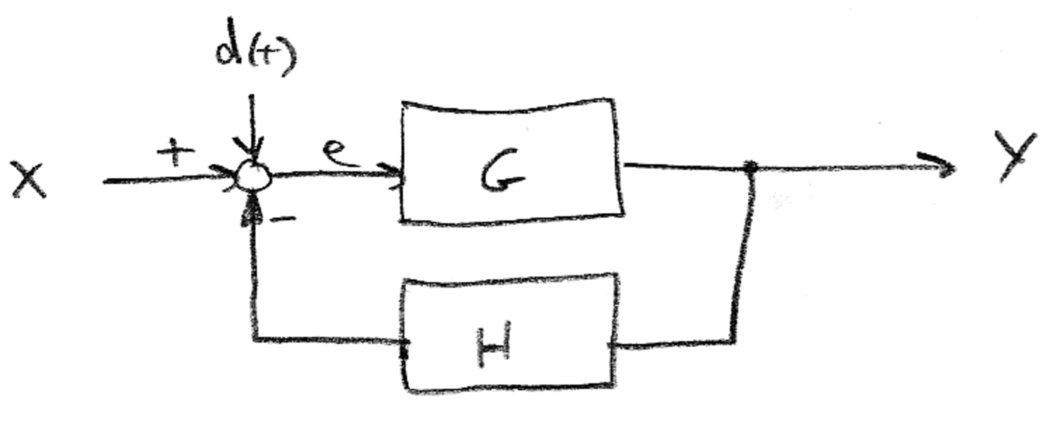
\includegraphics[width=3.5in]{figs06/00776a.png}
\caption{A closed loop negative feedback control system with a disturbance injected at the input.}\label{disturbanceaterror}
\end{figure}

\[
Y = GE = G(X+D-YH)
\]
\[
Y(1+GH) = GX + GD
\]
\[
Y = \frac{G}{1+GH}X  + \frac{G}{1+GH}D = \frac{G}{1+GH}(X+D)
\]

In this case the disturbance and the input are treated exactly the same. There is no disturbance rejection at all.  In retrospect this makes sense since it would be impossible for the controller to distinguish between the disturbance and the desired input.

Now we consider a case in which ``$G$" is split into two systems and the disturbance is injected between the two (Figure \ref{disturbancebetweenCP}).  As mentioned above,  this is an important case where $G$ consists of a controller coupled to a ``plant" such as an industrial machine or a vehicle.


\begin{figure}\centering
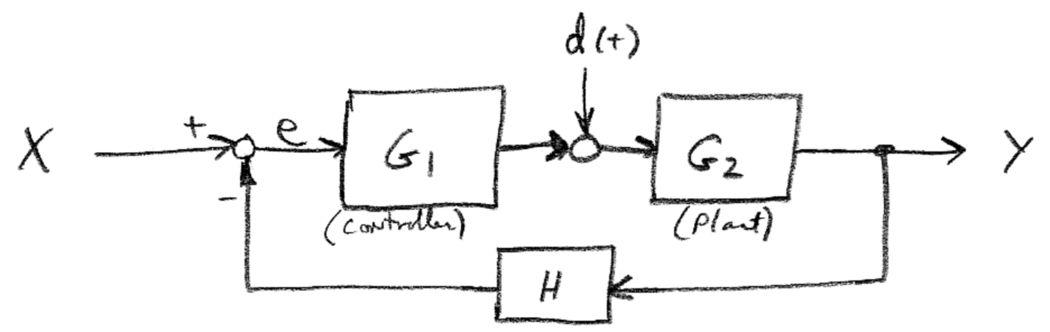
\includegraphics[width=3.5in]{figs06/00777a.png}
\caption{A closed loop negative feedback control system with a disturbance injected between the controller ($G_1$) and the plant $G_2$).}\label{disturbancebetweenCP}
\end{figure}


This time we have
\[
Y = G_2(D+G_1E)
\]
\[
= G_2\left ( D+G_1(X-YH) \right )
\]
\[
Y = G_2D + G_1G_2X - YG_1G_2H
\]
\[
Y(1+G_1G_2H) = G_2D + G_1G_2X
\]
\[
Y = \frac{G_2D}{1+G_1G_2H}  +  \frac{G_1G_2X}{1+G_1G_2H}
\]
Considering the case of a large loop gain, $G_1G_2H >> 1$, we have the situation where the disturbance is reduced by $G_1H$, which can be more or less disturbance rejection than reduction by $G_1G_2H$.





\begin{ExampleSmall}\label{stepdisturbanceexample}

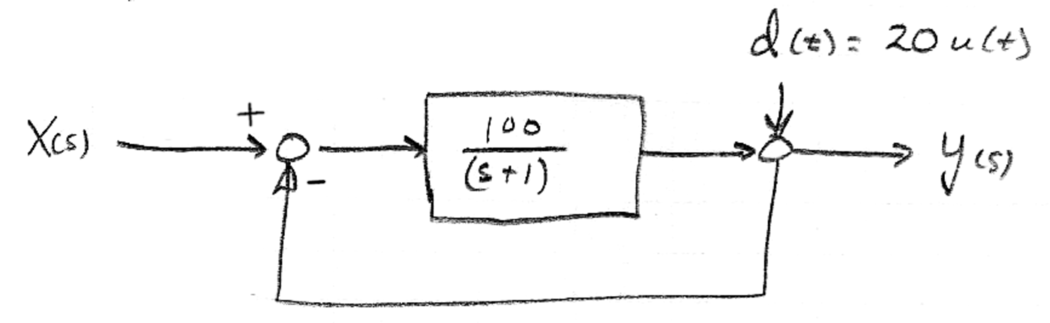
\includegraphics[width=3.5in]{figs06/00778a.png}

As a final example, for the system above, find $Y(s)$ and $y(t) = L^{-1} \left \{ Y(s) \right \}$ for $x(t) = 0$, $X(s) = 0$, $d(t) = 20u(t)$.

\vspace{0.25in}

\[
Y(s) = \frac{G}{1+GH}X(s) +  \frac{1}{1+GH}D(s)
\]
Since $X(s) = 0$, and the Laplace transform of $20u(t)$ is $20/s$,
\[
Y(s) = \frac{1}{1+\frac{100}{(s+1)}} D(s)  = \frac{(s+1)}{(s+101)} 20/s
\]
Expanding this with partial fractions
\[
\frac{20(s+1)}{s(s+101)} =  \frac{A_1}{s} +  \frac{A_2}{(s+101)}
\]
\[
A_1 = \left . \frac{20(s+1)}{(s+101)}\right | _{s=0} = \frac{20}{101} \approx 0.2
\]
\[
A_2 = \left . \frac{20(s+1)}{s}\right | _{s-101} = \frac{-2000}{-101} \approx 20
\]
Applying the inverse transform,
\[
y(t) = 0.2u(t) + 20e^{-101t}
\]

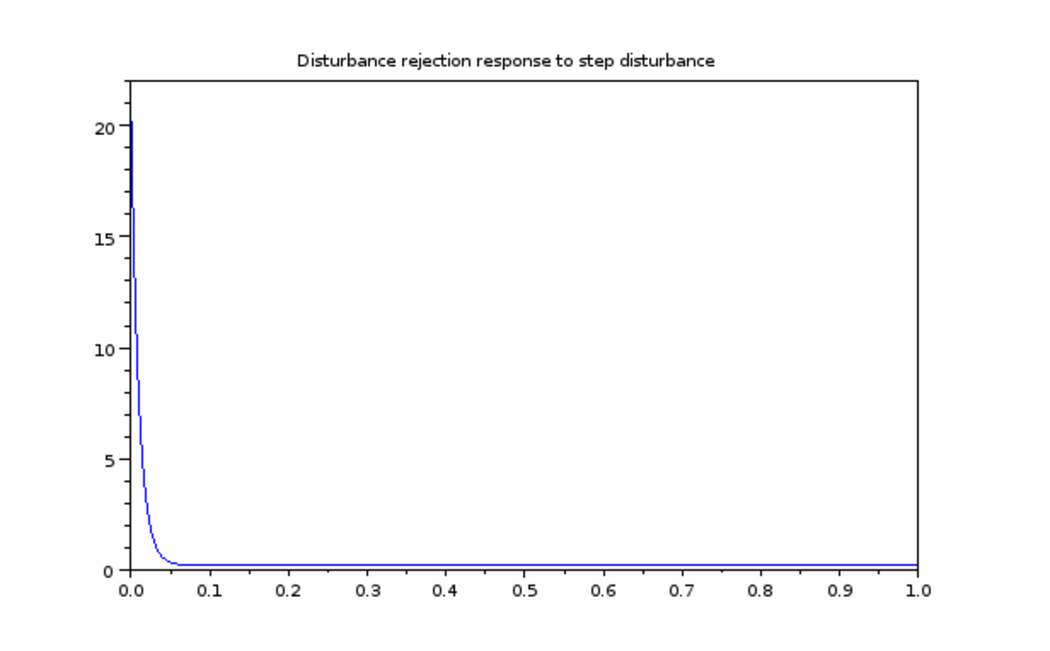
\includegraphics[width=3.5in]{figs06/stepdisturba.png}

The disturbance is reduced by about a factor of 100!   Note however that the second term is a transient arising from the step input of the disturbance.  Although this transient is over very quickly ($e^{-101t}$) it has a significant amplitude (20).   Disturbance rejection cannot react instantly!


\end{ExampleSmall}


\section{Stability}\label{FeedbackStabilitySection}


\begin{figure}\centering
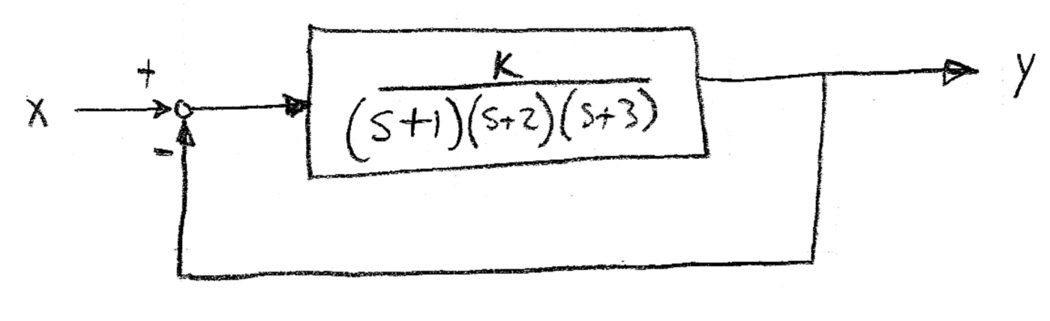
\includegraphics[width=3.5in]{figs06/00779a.png}
\caption{A closed loop negative feedback system with stable poles in the feed-forward path. $K$ is a positive real constant, a gain.}\label{openloopstable}
\end{figure}

We've seen many systems like that of Example \thechapter.\ref{stepdisturbanceexample}, which contain transient solutions with exponential terms.
The time coefficient on the exponential terms comes from the real part of poles.
As long as the poles have a negative real part (i.e. they are in the left half of the complex plane)
the system will converge to a steady value.
Because of the negative term, all the exponentials fade out to zero with time.

On the other hand, if the time coefficient (real part of the pole) is positive, even for only one of the exponential terms arising from the partial fraction expansion, the output will grow exponentially without limit.  In almost all practical systems this is unacceptable and undesirable.

\subsection{Calculation of Roots}\label{calculationofroots}

At first glance it seems stability is trivial to assess.  If any poles have positive real parts, the system is unstable.  The tricky part comes from closed loop negative feedback systems.   Consider the system of Figure \ref{openloopstable}.  In our terminology,
\[
G(s) =  \frac  {K}  {(s+1)(s+2)(s+3)}
\]
where $K$ is a positive real constant (we refer to terms like $K$ as a {\it gain}) and $H=1$.
Clearly $G(s)$ is stable since the poles are $s=\{-1, -2, -3\}$.
But what about when we consider the closed loop gain
\[
\frac{Y(s)}{X(s)} =  \frac{\frac{K}{(s+1)(s+2)(s+3)}}  {1+ \frac  {K}  {(s+1)(s+2)(s+3)}}
\]
?
\noindent
Multiplying through by the poles of $G(s)$ we get
\[
= \frac {K}  {(s+1)(s+2)(s+3) + K}
\]
The denominator $(s+1)(s+2)(s+3) + K$ is called the characteristic equation and it has different roots than the poles of $G(s)$.   For our closed loop transfer function, the poles are solutions to
\[
s^3+6s^2+11s+6 +K = 0
\]
Below are the roots of this characteristic polynomial, solved by computer for various values of $K$:

\begin{verbatim}
K=0.0
  - 3.  - 2.  - 1.
K=2.0
  - 3.5213797,   - 1.2393101 - 0.8578736i,  - 1.2393101 + 0.8578736i
K=4.0
  - 3.7963219,   - 1.101839 - 1.1916708i,   - 1.101839 + 1.1916708i
K=6.0
  - 4.           - 1.       - 1.4142136i,   - 1. + 1.4142136i
K=8.0
  - 4.1663127   - 0.9168436 - 1.587351i     - 0.9168436 + 1.587351i
K-10.0
  - 4.3089073,  - 0.8455463 - 1.731557i,    - 0.8455463 + 1.731557i
K=20.0
  - 4.8371387,  - 0.5814307 - 2.2443299i,   - 0.5814307 + 2.2443299i
K=30.0
  - 5.214468,   - 0.3927660 - 2.5979998i,   - 0.3927660 + 2.5979998i
K=40.0
  - 5.5173935,  - 0.2413032 - 2.8773326i,   - 0.2413032 + 2.8773326i
K=50.0
  - 5.7744943,  - 0.1127528 - 3.1120902i,   - 0.1127528 + 3.1120902i
K=60.0
  - 6.,           1.665D-15 - 3.3166248i,      1.665D-15 + 3.3166248i
K=70.0
  - 6.202156,     0.1010780 - 3.4990837i,      0.1010780 + 3.4990837i
K=80.0
  - 6.386221,     0.1931105 - 3.6645875i,      0.1931105 + 3.6645875i
K=90.0
  - 6.5557795,    0.2778897 - 3.8165881i,      0.2778897 + 3.8165881i
K=100.0
  - 6.7133977,    0.3566988 - 3.9575356i       0.3566988 + 3.9575356i

\end{verbatim}

Notice two main points:

\begin{itemize}
  \item When $K=0$ (first line) the closed loop poles are the same as the open loop poles.
  \item At $K=2.0$ two of the poles become complex conjugates (CC) whereas they were all real for $K=0$.
  \item When $K=60$ the real part of the CC poles is essentially zero.
  \item The real part of the CC poles becomes positive for $K>60$.
\end{itemize}


 From these observations we can conclude that the system is stable for gains below 60 but unstable for gains above that.  While this is a simple analysis to perform with the computer, in the early days of control engineering,  predicting stability of a closed loop system
 was a major challenge because of the lack of practical manual methods for solving polynomials above order 2.
 This was true even when each block was fully and accurately modeled.
 In response, some clever manual  techniques were developed for stability analyis and some of those are still important today, especially during design.



\section{Stability in the Frequency Domain}



The following is a very basic derivation of closed loop stability.  It applies only to systems whos blocks have only poles with negative real parts or poles at the origin.

Consider the closed loop system of Figure \ref{NyquistLoop}, Left.  Recall that any function of $s$ has a complex value which in turn has an angle and magnitude.  Suppose we look at the steady state sinusoidal domain ($s=j\omega$, see Section \ref{FrequencyResponseSection}) and further suppose that for some $\omega$,

$$
\angle A(j\omega) = 180^\circ
$$
This would have the effect of changing the sign on the feedback loop and causing ``positive
 feedback" also known as instability.


Suppose on the other hand that $A$ is real (i.e. $\angle A = 0$) but we add a term of $H=-1$ to the feedback loop (Figure \ref{NyquistLoop}, Right).  In both of these cases the total angle around the loop (the angle of the loop gain) is $180^\circ$.    Analyzing the closed loop gain
\[
Y = A(X-(-Y)) = AX + AY
\]
\[
\frac{Y}{X}  = \frac {A} {1-A}
\]
for the case $A=1$,
\[
|\frac{Y}{X}| \to \infty
\]


\begin{figure}\centering
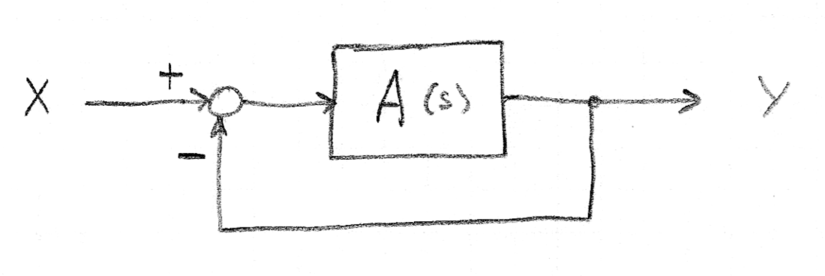
\includegraphics[width=2.75in]{figs06/00792a.png}
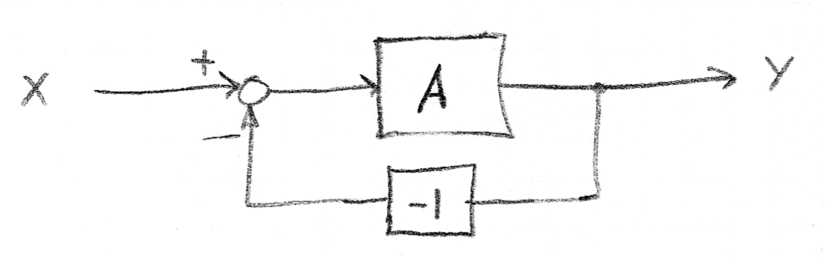
\includegraphics[width=2.75in]{figs06/00793a.png}
% \caption{If $\angle A(s) = 180^\circ$ the gain around the loop becomes positive.}\label{NyquistLoop}
\caption{If the phase angle of $A(s)$ is 180$^\circ$, the gain around the loop becomes positive.}\label{NyquistLoop}
\end{figure}

Lets expand $A(s) = C(s)P(s)$ to represent the combination of controller ($C(s)$) and
plant ($P(s)$). Then, if the loop gain is $M(s) = C(s)P(s)H(s)$, a condition on the loop gain for instability is
\[
\left | M(j\omega) \right | = 1, \qquad \angle M(j\omega) = 180^\circ
\]

Using the BAMP we should be able to detect this combination.

\begin{ExampleSmall}\label{bodestabilityexample}
A system has the closed loop transfer function
\[
G(s) = \frac {3.9\times 10^4} {(s+1)(s+22)(s+100)}
\]

Use the Bode magnitude and phase plots to check the closed loop stability.

Drawing the Bode plots,

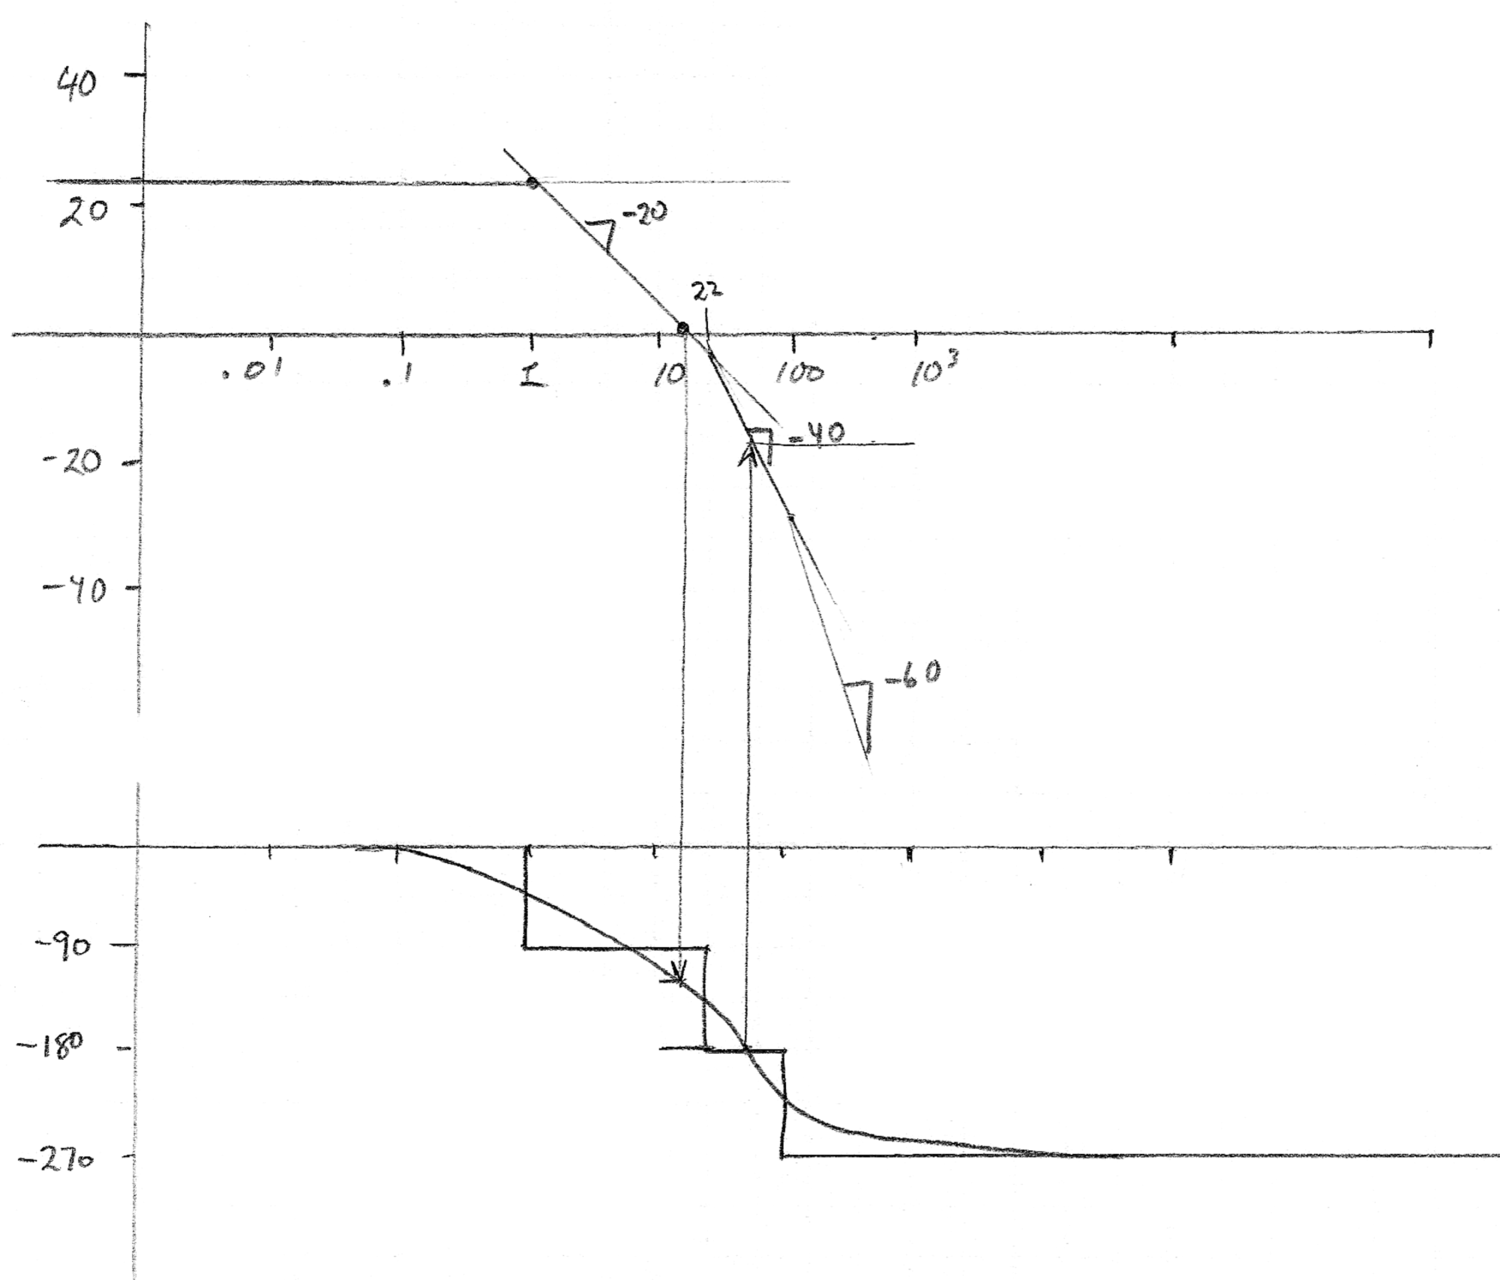
\includegraphics[width=5.0in]{figs06/00794aa.png}

We first identify the point where the BAMP crosses 0$dB$ (magnitude = 1), then we find the phase angle by reading the phase plot at the same frequency (about 10.5 rad/sec).   This is illustrated graphically by a vertical line dropping down from the $0dB$ axis to the phase plot.  Reading that value we get a phase angle of about $120^\circ$.  This is well short of $180^\circ$ so the system is stable.

Another way to evaluate stability is to look at where the phase curve crosses $180^\circ$ and evaluate gain.  In this case we find that the phase curve crosses $180^\circ$ at about $\omega=60$.  Going straight up from the phase to the magnitude curve, we find the magnitude at $\omega = 60$ is about $-16dB$, also indicating a stable system.
\end{ExampleSmall}

\subsection{Gain and Phase Margins}\label{GainPhaseMargins}

In Example \thechapter.\ref{bodestabilityexample}, when we looked at the frequency where magnitude was 1, we had a phase of $120^\circ$.  The criterion for instability is $180^\circ$ so we have a {\it margin} of $60^\circ$ before stability is lost.  Similarly, when we look at the frequency where angle was $180^\circ$, we got a magnitude of $-16dB$ so our margin is $16dB$ before gain magnitude is 1.   These margins are important because they are the degree of safety we have in the face of possible changes in magnitude or phase due to changes in parameters which might happen due to real-world factors such as wear and tear.   We thus define

\begin{itemize}
  \item {\bf Gain  Margin:} at the frequency where $\angle CPH(s) = 180^\circ$, the difference in $dB$ between the loop gain magnitude and 0$dB$.  A positive gain margin indicates stability:
  the loop gain could increase by that much before getting greater than $0dB$.
  \item {\bf Phase Margin:} at the frequency where $\left |CPH(s) = 1\right |$, the difference in degrees  between the phase plot and $180^\circ$.
\end{itemize}


\begin{ExampleSmall}
For the system and Bode plots of Example \thechapter.\ref{bodestabilityexample}, find the Gain and Phase Margins.

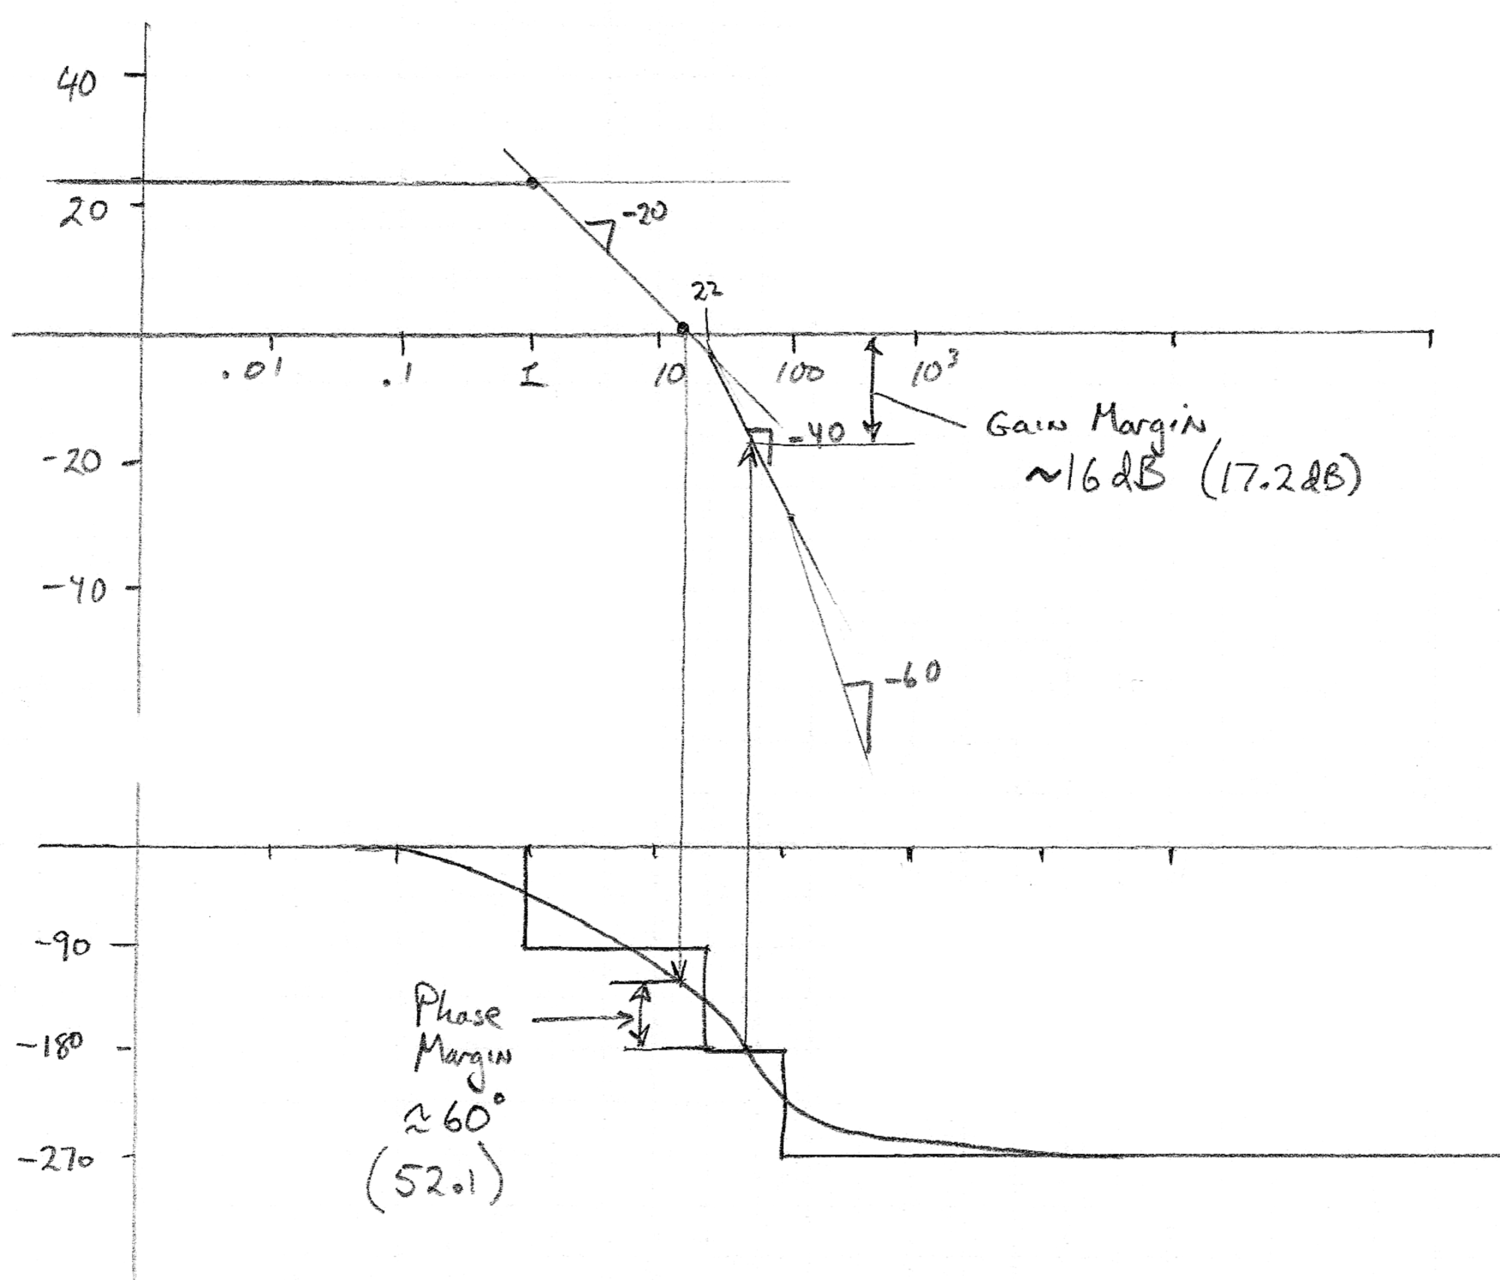
\includegraphics[width=5.0in]{figs06/00794a.png}

The gain and phase margins are simply added on to the Bode Magnitude and phase plots.

\end{ExampleSmall}

\begin{ExampleSmall}
Find the Gain and Phase Margins for
\[
G_2(s) = \frac  {4\times10^5}  {(s+1)(s+31.6)(s+100)}
\]
Carefully drawing the Bode gain and phase plots by hand:

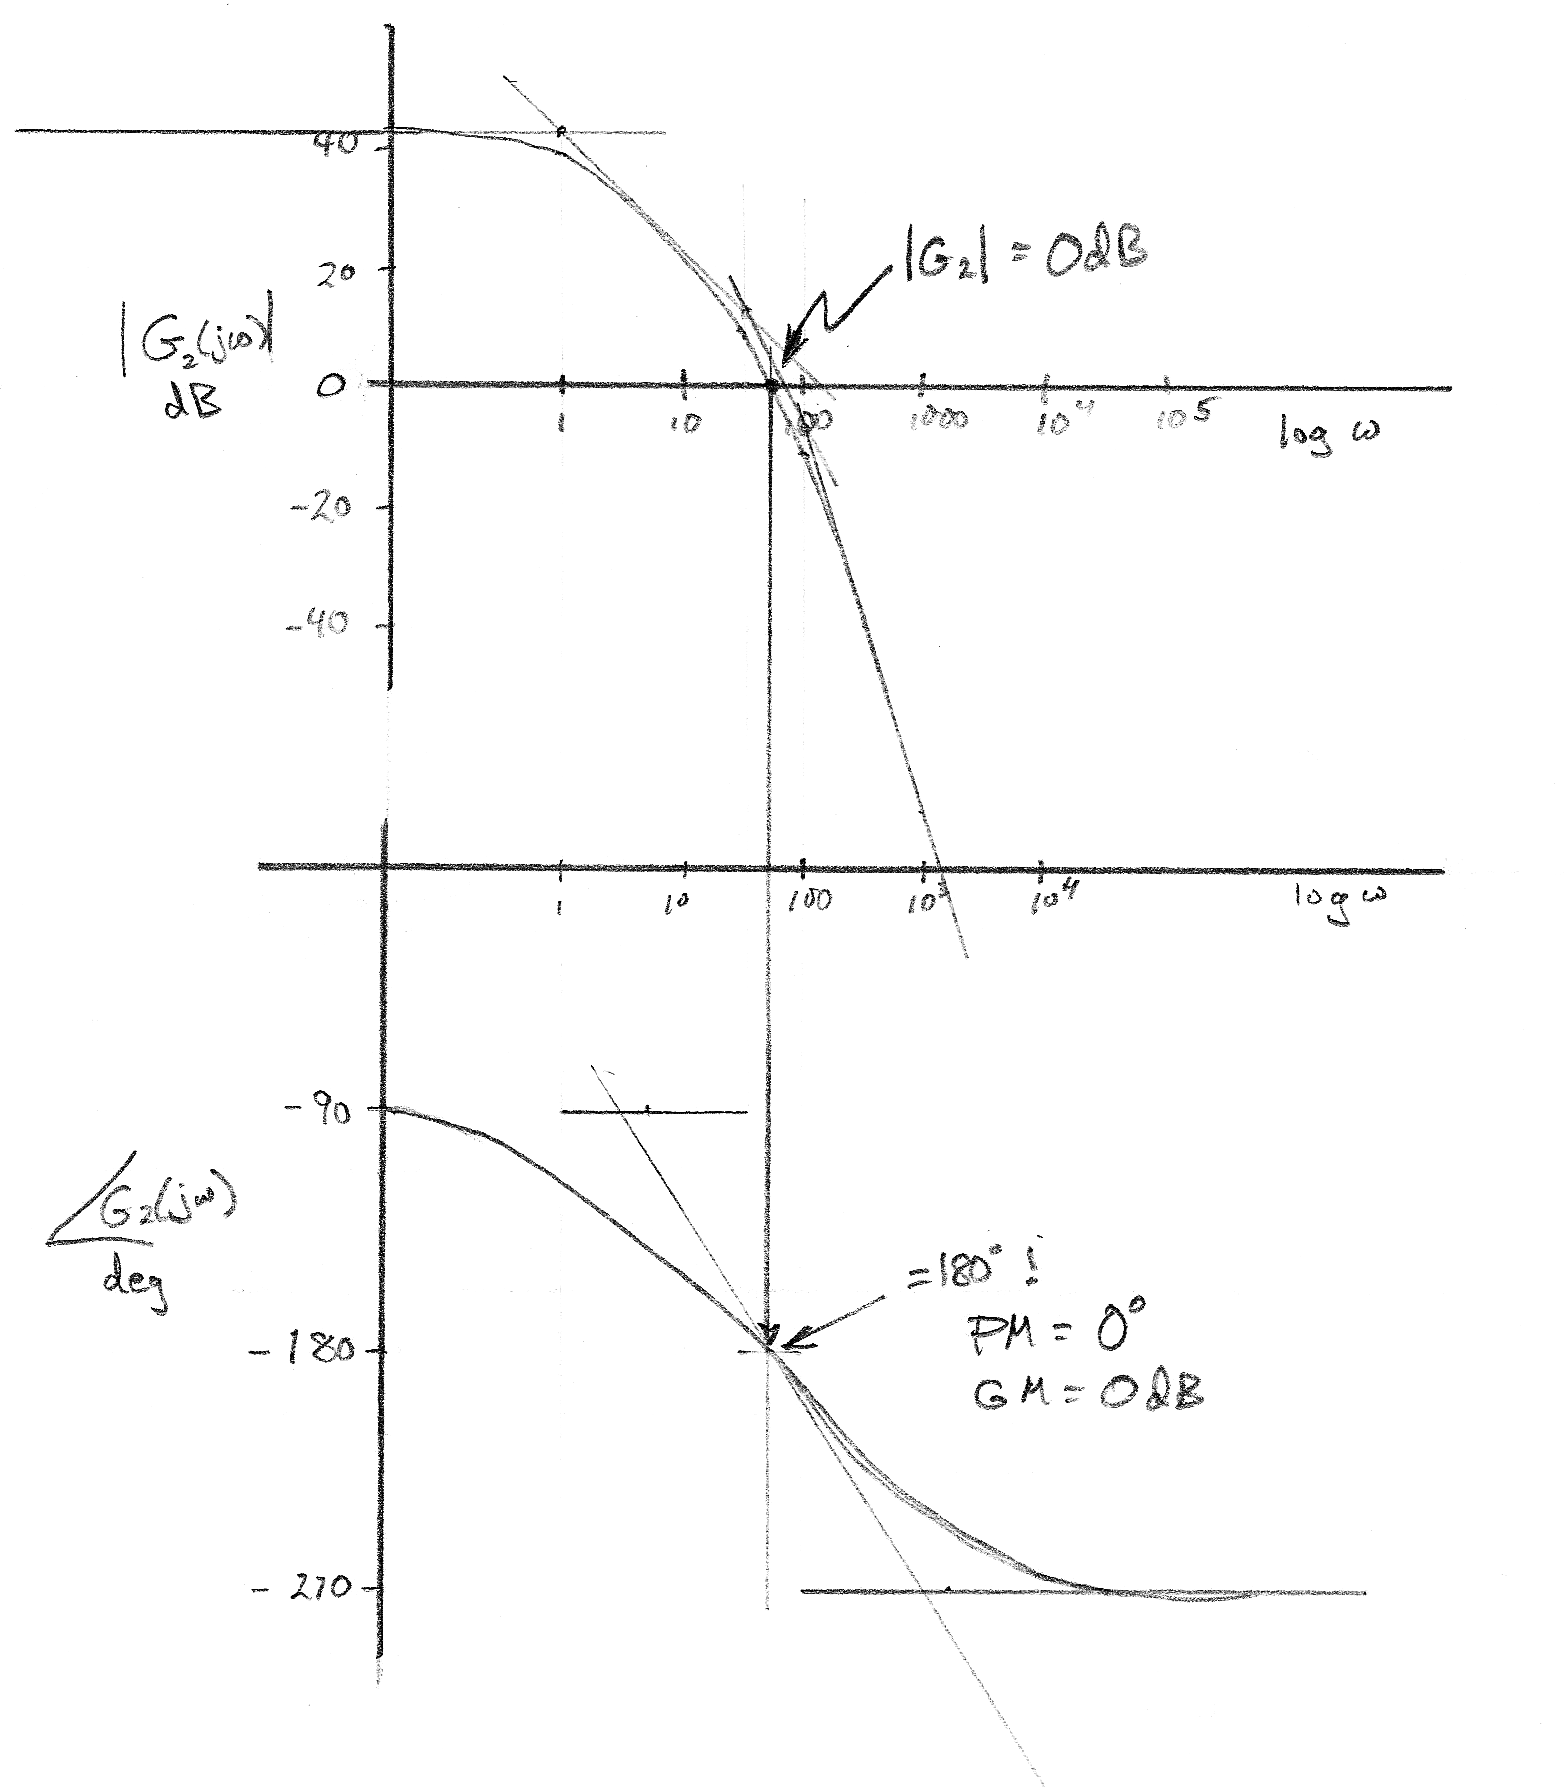
\includegraphics[width=110mm]{figs06/01063.png}

Using pencil and paper we get Gain and Phase margins of 0.  This means the system is right on the edge.  Certainly with
the limited precision of pencil work, we would be safe to consider this unstable.
Using python.control's {\tt  margin()} command we get more precisely:
\[
GM = 0.69dB \qquad PM = 2.0^\circ
\]
Because we never know the system parameters with high accuracy, these margins would not be considered safe.
\end{ExampleSmall}
% \section{Summary of Notation}

























